% Options for packages loaded elsewhere
\PassOptionsToPackage{unicode}{hyperref}
\PassOptionsToPackage{hyphens}{url}
%
\documentclass[
]{scrbook}
\usepackage{amsmath,amssymb}
\usepackage{iftex}
\ifPDFTeX
  \usepackage[T1]{fontenc}
  \usepackage[utf8]{inputenc}
  \usepackage{textcomp} % provide euro and other symbols
\else % if luatex or xetex
  \usepackage{unicode-math} % this also loads fontspec
  \defaultfontfeatures{Scale=MatchLowercase}
  \defaultfontfeatures[\rmfamily]{Ligatures=TeX,Scale=1}
\fi
\usepackage{lmodern}
\ifPDFTeX\else
  % xetex/luatex font selection
\fi
% Use upquote if available, for straight quotes in verbatim environments
\IfFileExists{upquote.sty}{\usepackage{upquote}}{}
\IfFileExists{microtype.sty}{% use microtype if available
  \usepackage[]{microtype}
  \UseMicrotypeSet[protrusion]{basicmath} % disable protrusion for tt fonts
}{}
\makeatletter
\@ifundefined{KOMAClassName}{% if non-KOMA class
  \IfFileExists{parskip.sty}{%
    \usepackage{parskip}
  }{% else
    \setlength{\parindent}{0pt}
    \setlength{\parskip}{6pt plus 2pt minus 1pt}}
}{% if KOMA class
  \KOMAoptions{parskip=half}}
\makeatother
\usepackage{xcolor}
\usepackage{longtable,booktabs,array}
\usepackage{calc} % for calculating minipage widths
% Correct order of tables after \paragraph or \subparagraph
\usepackage{etoolbox}
\makeatletter
\patchcmd\longtable{\par}{\if@noskipsec\mbox{}\fi\par}{}{}
\makeatother
% Allow footnotes in longtable head/foot
\IfFileExists{footnotehyper.sty}{\usepackage{footnotehyper}}{\usepackage{footnote}}
\makesavenoteenv{longtable}
\usepackage{graphicx}
\makeatletter
\def\maxwidth{\ifdim\Gin@nat@width>\linewidth\linewidth\else\Gin@nat@width\fi}
\def\maxheight{\ifdim\Gin@nat@height>\textheight\textheight\else\Gin@nat@height\fi}
\makeatother
% Scale images if necessary, so that they will not overflow the page
% margins by default, and it is still possible to overwrite the defaults
% using explicit options in \includegraphics[width, height, ...]{}
\setkeys{Gin}{width=\maxwidth,height=\maxheight,keepaspectratio}
% Set default figure placement to htbp
\makeatletter
\def\fps@figure{htbp}
\makeatother
\setlength{\emergencystretch}{3em} % prevent overfull lines
\providecommand{\tightlist}{%
  \setlength{\itemsep}{0pt}\setlength{\parskip}{0pt}}
\setcounter{secnumdepth}{5}
% definitions for citeproc citations
\NewDocumentCommand\citeproctext{}{}
\NewDocumentCommand\citeproc{mm}{%
  \begingroup\def\citeproctext{#2}\cite{#1}\endgroup}
\makeatletter
 % allow citations to break across lines
 \let\@cite@ofmt\@firstofone
 % avoid brackets around text for \cite:
 \def\@biblabel#1{}
 \def\@cite#1#2{{#1\if@tempswa , #2\fi}}
\makeatother
\newlength{\cslhangindent}
\setlength{\cslhangindent}{1.5em}
\newlength{\csllabelwidth}
\setlength{\csllabelwidth}{3em}
\newenvironment{CSLReferences}[2] % #1 hanging-indent, #2 entry-spacing
 {\begin{list}{}{%
  \setlength{\itemindent}{0pt}
  \setlength{\leftmargin}{0pt}
  \setlength{\parsep}{0pt}
  % turn on hanging indent if param 1 is 1
  \ifodd #1
   \setlength{\leftmargin}{\cslhangindent}
   \setlength{\itemindent}{-1\cslhangindent}
  \fi
  % set entry spacing
  \setlength{\itemsep}{#2\baselineskip}}}
 {\end{list}}
\usepackage{calc}
\newcommand{\CSLBlock}[1]{\hfill\break\parbox[t]{\linewidth}{\strut\ignorespaces#1\strut}}
\newcommand{\CSLLeftMargin}[1]{\parbox[t]{\csllabelwidth}{\strut#1\strut}}
\newcommand{\CSLRightInline}[1]{\parbox[t]{\linewidth - \csllabelwidth}{\strut#1\strut}}
\newcommand{\CSLIndent}[1]{\hspace{\cslhangindent}#1}
\usepackage{booktabs} % for better tables

% fonts
% libertine font: https://www.tug.org/FontCatalogue/linuxlibertine/
\usepackage[oldstyle]{libertine}
\usepackage{libertinust1math}
% \usepackage[T1]{fontenc}
\usepackage[extralight]{inter} 

\usepackage[left=3cm, right=2.5cm, top=2.5cm, bottom=4cm]{geometry} % page margings

\usepackage{tabto} % for aligning text at a certain position, used for title page

\usepackage[ngerman, english]{babel}		% main language is the last in the list, more infor is here: https://en.wikibooks.org/wiki/LaTeX/Internationalization#Babel

\usepackage[onehalfspacing]{setspace}	% clean 1.5 leading / spacing
\RedeclareSectionCommand[beforeskip=0.5em,afterskip=2em]{chapter} % define space before and after heading

\usepackage{pdfpages} % to include pdfs
\ifLuaTeX
  \usepackage{selnolig}  % disable illegal ligatures
\fi
\usepackage{bookmark}
\IfFileExists{xurl.sty}{\usepackage{xurl}}{} % add URL line breaks if available
\urlstyle{same}
\hypersetup{
  hidelinks,
  pdfcreator={LaTeX via pandoc}}

\author{}
\date{\vspace{-2.5em}}

\begin{document}

\frontmatter

\begin{titlepage}                   
    \begin{center}
        
\includegraphics[height=3.2cm]{logo.pdf}\\[40mm]
        
        \huge {\linespread{1.5} Rethinking Variation in Social Cognition: \\ Gaze Following across Individuals, Ages, and Communities}\\[30mm]
        
                
        \normalsize Von der Fakultät Nachhaltigkeit \\ der Leuphana Universität Lüneburg zur Erlangung des Grades\\
        Doktorin der Psychologie\\-- Dr. rer. nat. --\\[10mm]
        
        genehmigte Dissertation von\\[10mm]
        Julia Christin Prein\\
        geboren am TT.MM.JJJJ in XXX
        
    \vspace*{\fill} 
    \end{center}
    
    \newpage
    \thispagestyle{empty}
    \begin{flushleft}
      \begin{normalsize}
      
      \vspace*{\fill} 
            Eingereicht am: \tabto*{30mm} 1. Oktober 2024 \\[10mm]
            
            Erstbetreuer: \tabto*{30mm} Prof.\,Dr.\, Manuel Bohn, \textit{Leuphana Universität Lüneburg}\\
                Zweitbetreuer: \tabto*{30mm} Prof.\,Dr.\, Sebastian Wallot, \textit{Leuphana Universität Lüneburg}\\[10mm]
                
                Erstgutachter: \tabto*{30mm} Prof.\,Dr.\, Manuel Bohn, \textit{Leuphana Universität Lüneburg}\\
                Zweitgutachter: \tabto*{30mm} Prof.\,Dr.\, Sebastian Wallot, \textit{Leuphana Universität Lüneburg}\\
                Drittgutachter: \tabto*{30mm} Prof.\,Dr.\, Daniel Haun, \textit{Universität Leipzig \& Max-Planck-Institut für\\
                \tabto*{30mm} Evolutionäre Anthropologie}\\[10mm]
        \end{normalsize}
    \end{flushleft}
    
\end{titlepage}

\tableofcontents

\chapter{Copyright Notice}\label{copyright}

The research articles included in this cumulative dissertation have been or will be published in international peer-reviewed journals. Copyright of the text and illustrations lies with the author or authors of the respective chapter(s). The publishers own the exclusive rights to publish or use the text and illustrations for their own purposes. Reprinting any part of this dissertation thesis requires the permission of the copyright holder(s).
The individual contributions of this cumulative thesis have been or will be published (in chronological order) as follows:

Prein, J. C., Kalinke, S., Haun, D. B. M.*, \& Bohn, M.* (2023). TANGO: A reliable, open-source, browser-based task to assess individual differences in gaze understanding in 3 to 5-year-old children and adults. \emph{Behavior Research Methods, 56}(3), 2469--2485. \url{https://doi.org/10.3758/s13428-023-02159-5}

Prein, J. C., Maurits, L., Werwach, A., Haun, D. B. M.,* \& Bohn, M.* (2024). \emph{Variation in gaze understanding across the life span: A process-level perspective.} PsyArXiv. \url{https://doi.org/10.31234/osf.io/dy73a}

Bohn, M.*, Prein, J. C.*, Ayikoru, A., Bednarski, F. M., Dzabatou, A., Frank, M. C., Henderson, A. M. E., Isabella, J., Kalbitz, J., Kanngiesser, P., Keşşafoğlu, D., Koymen, B., Manrique-Hernandez, M., Magazi, S., Mújica-Manrique, L., Ohlendorf, J., Olaoba, D., Pieters, W., Pope-Caldwell, S., \ldots{} Haun, D. (2024). \emph{A universal of human social cognition: Children from 17 communities process gaze in similar ways.} PsyArXiv. \url{https://doi.org/10.31234/osf.io/z3ahv}

Prein, J. C., Maurits, L., Werwach, A., Haun, D. B. M., \& Bohn, M. (2024). \emph{Variation in gaze following across the life span: A process-level perspective.} PsyArXiv. \url{https://doi.org/10.31234/osf.io/dy73a}

~

Further articles that were written in the context of this dissertation can be found in the Appendix and have been or will be published as follows (in chronological order):

Schuwerk, T., Kampis, D., Baillargeon, R., Biro, S., Bohn, M., Byers-Heinlein, K., Dörrenberg, S., Fisher, C., Franchin, L., Fulcher, T., Garbisch, I., Geraci, A., Grosse Wiesmann, C., Hamlin, K., Haun, D. B. M., Hepach, R., Hunnius, S., Hyde, D. C., Karman, P., \ldots, Prein, J., \ldots{} Rakoczy, H. (2021). \emph{Action anticipation based on an agent's epistemic state in toddlers and adults. Child Development} (In-Principle Acceptance of Registered Report Stage 1: Study Design). PsyArXiv. \url{https://doi.org/10.31234/osf.io/x4jbm}

Bohn, M., Prein, J. C., Engicht, J., Haun, D., Gagarina, N., \& Koch, T. (2023). \emph{PREVIC: An adaptive parent report measure of expressive vocabulary in children between 3 and 8 years of age.} PsyArXiv. \url{https://doi.org/10.31234/osf.io/hvncp}

Bohn, M.*, Prein, J.*, Koch, T., Bee, R. M., Delikaya, B., Haun, D., \& Gagarina, N. (2024). oREV: An item response theory-based open receptive vocabulary task for 3- to 8-year-old children. \emph{Behavior Research Methods, 56}(3), 2595--2605. \url{https://doi.org/10.3758/s13428-023-02169-3}

Steffan, A., Zimmer, L., Arias-Trejo, N., Bohn, M., Dal Ben, R., Flores-Coronado, M. A., Franchin, L., Garbisch, I., Grosse Wiesmann, C., Hamlin, J. K., Havron, N., Hay, J. F., Hermansen, T. K., Jakobsen, K. V., Kalinke, S., Ko, E.-S., Kulke, L., Mayor, J., Meristo, M., \ldots, Prein, J., \ldots, Schuwerk, T. (2024). Validation of an open source, remote web-based eye-tracking method (WebGazer) for research in early childhood. \emph{Infancy, 29}(1), 31--55. \url{https://doi.org/10.1111/infa.12564}

~

* denotes shared first or last authorship.

\chapter{Abstract}\label{abstract}

Prein et al. (\citeproc{ref-prein2023tango}{2023})

Lorem ipsum dolor sit amet, consectetur adipiscing elit, sed do eiusmod tempor incididunt ut labore et dolore magna aliqua. Luctus venenatis lectus magna fringilla urna. Laoreet non curabitur gravida arcu ac tortor. Faucibus vitae aliquet nec ullamcorper sit amet risus nullam eget. Cras semper auctor neque vitae tempus quam pellentesque. Imperdiet massa tincidunt nunc pulvinar sapien et ligula ullamcorper. Et tortor at risus viverra adipiscing at. Congue nisi vitae suscipit tellus mauris. Habitant morbi tristique senectus et netus et malesuada fames ac. Eget mauris pharetra et ultrices neque. Aenean et tortor at risus viverra. Tempor orci dapibus ultrices in iaculis nunc sed augue. Euismod lacinia at quis risus sed vulputate odio ut enim. Id eu nisl nunc mi ipsum faucibus. Est lorem ipsum dolor sit amet. Eget velit aliquet sagittis id consectetur purus. Faucibus ornare suspendisse sed nisi. Pellentesque diam volutpat commodo sed egestas egestas fringilla.

\chapter{Zusammenfassung}\label{zusammenfassung}

Lorem ipsum dolor sit amet, consectetur adipiscing elit, sed do eiusmod tempor incididunt ut labore et dolore magna aliqua. Luctus venenatis lectus magna fringilla urna. Laoreet non curabitur gravida arcu ac tortor. Faucibus vitae aliquet nec ullamcorper sit amet risus nullam eget. Cras semper auctor neque vitae tempus quam pellentesque. Imperdiet massa tincidunt nunc pulvinar sapien et ligula ullamcorper. Et tortor at risus viverra adipiscing at. Congue nisi vitae suscipit tellus mauris. Habitant morbi tristique senectus et netus et malesuada fames ac. Eget mauris pharetra et ultrices neque. Aenean et tortor at risus viverra. Tempor orci dapibus ultrices in iaculis nunc sed augue. Euismod lacinia at quis risus sed vulputate odio ut enim. Id eu nisl nunc mi ipsum faucibus. Est lorem ipsum dolor sit amet. Eget velit aliquet sagittis id consectetur purus. Faucibus ornare suspendisse sed nisi. Pellentesque diam volutpat commodo sed egestas egestas fringilla.

\chapter{Danksagung}\label{danksagung}

\mainmatter

\chapter{Introduction}\label{introduction}

This will lead you to \hyperref[studyIII]{Study III}.

\section{How to include figures:}\label{how-to-include-figures}



\begin{figure}

{\centering 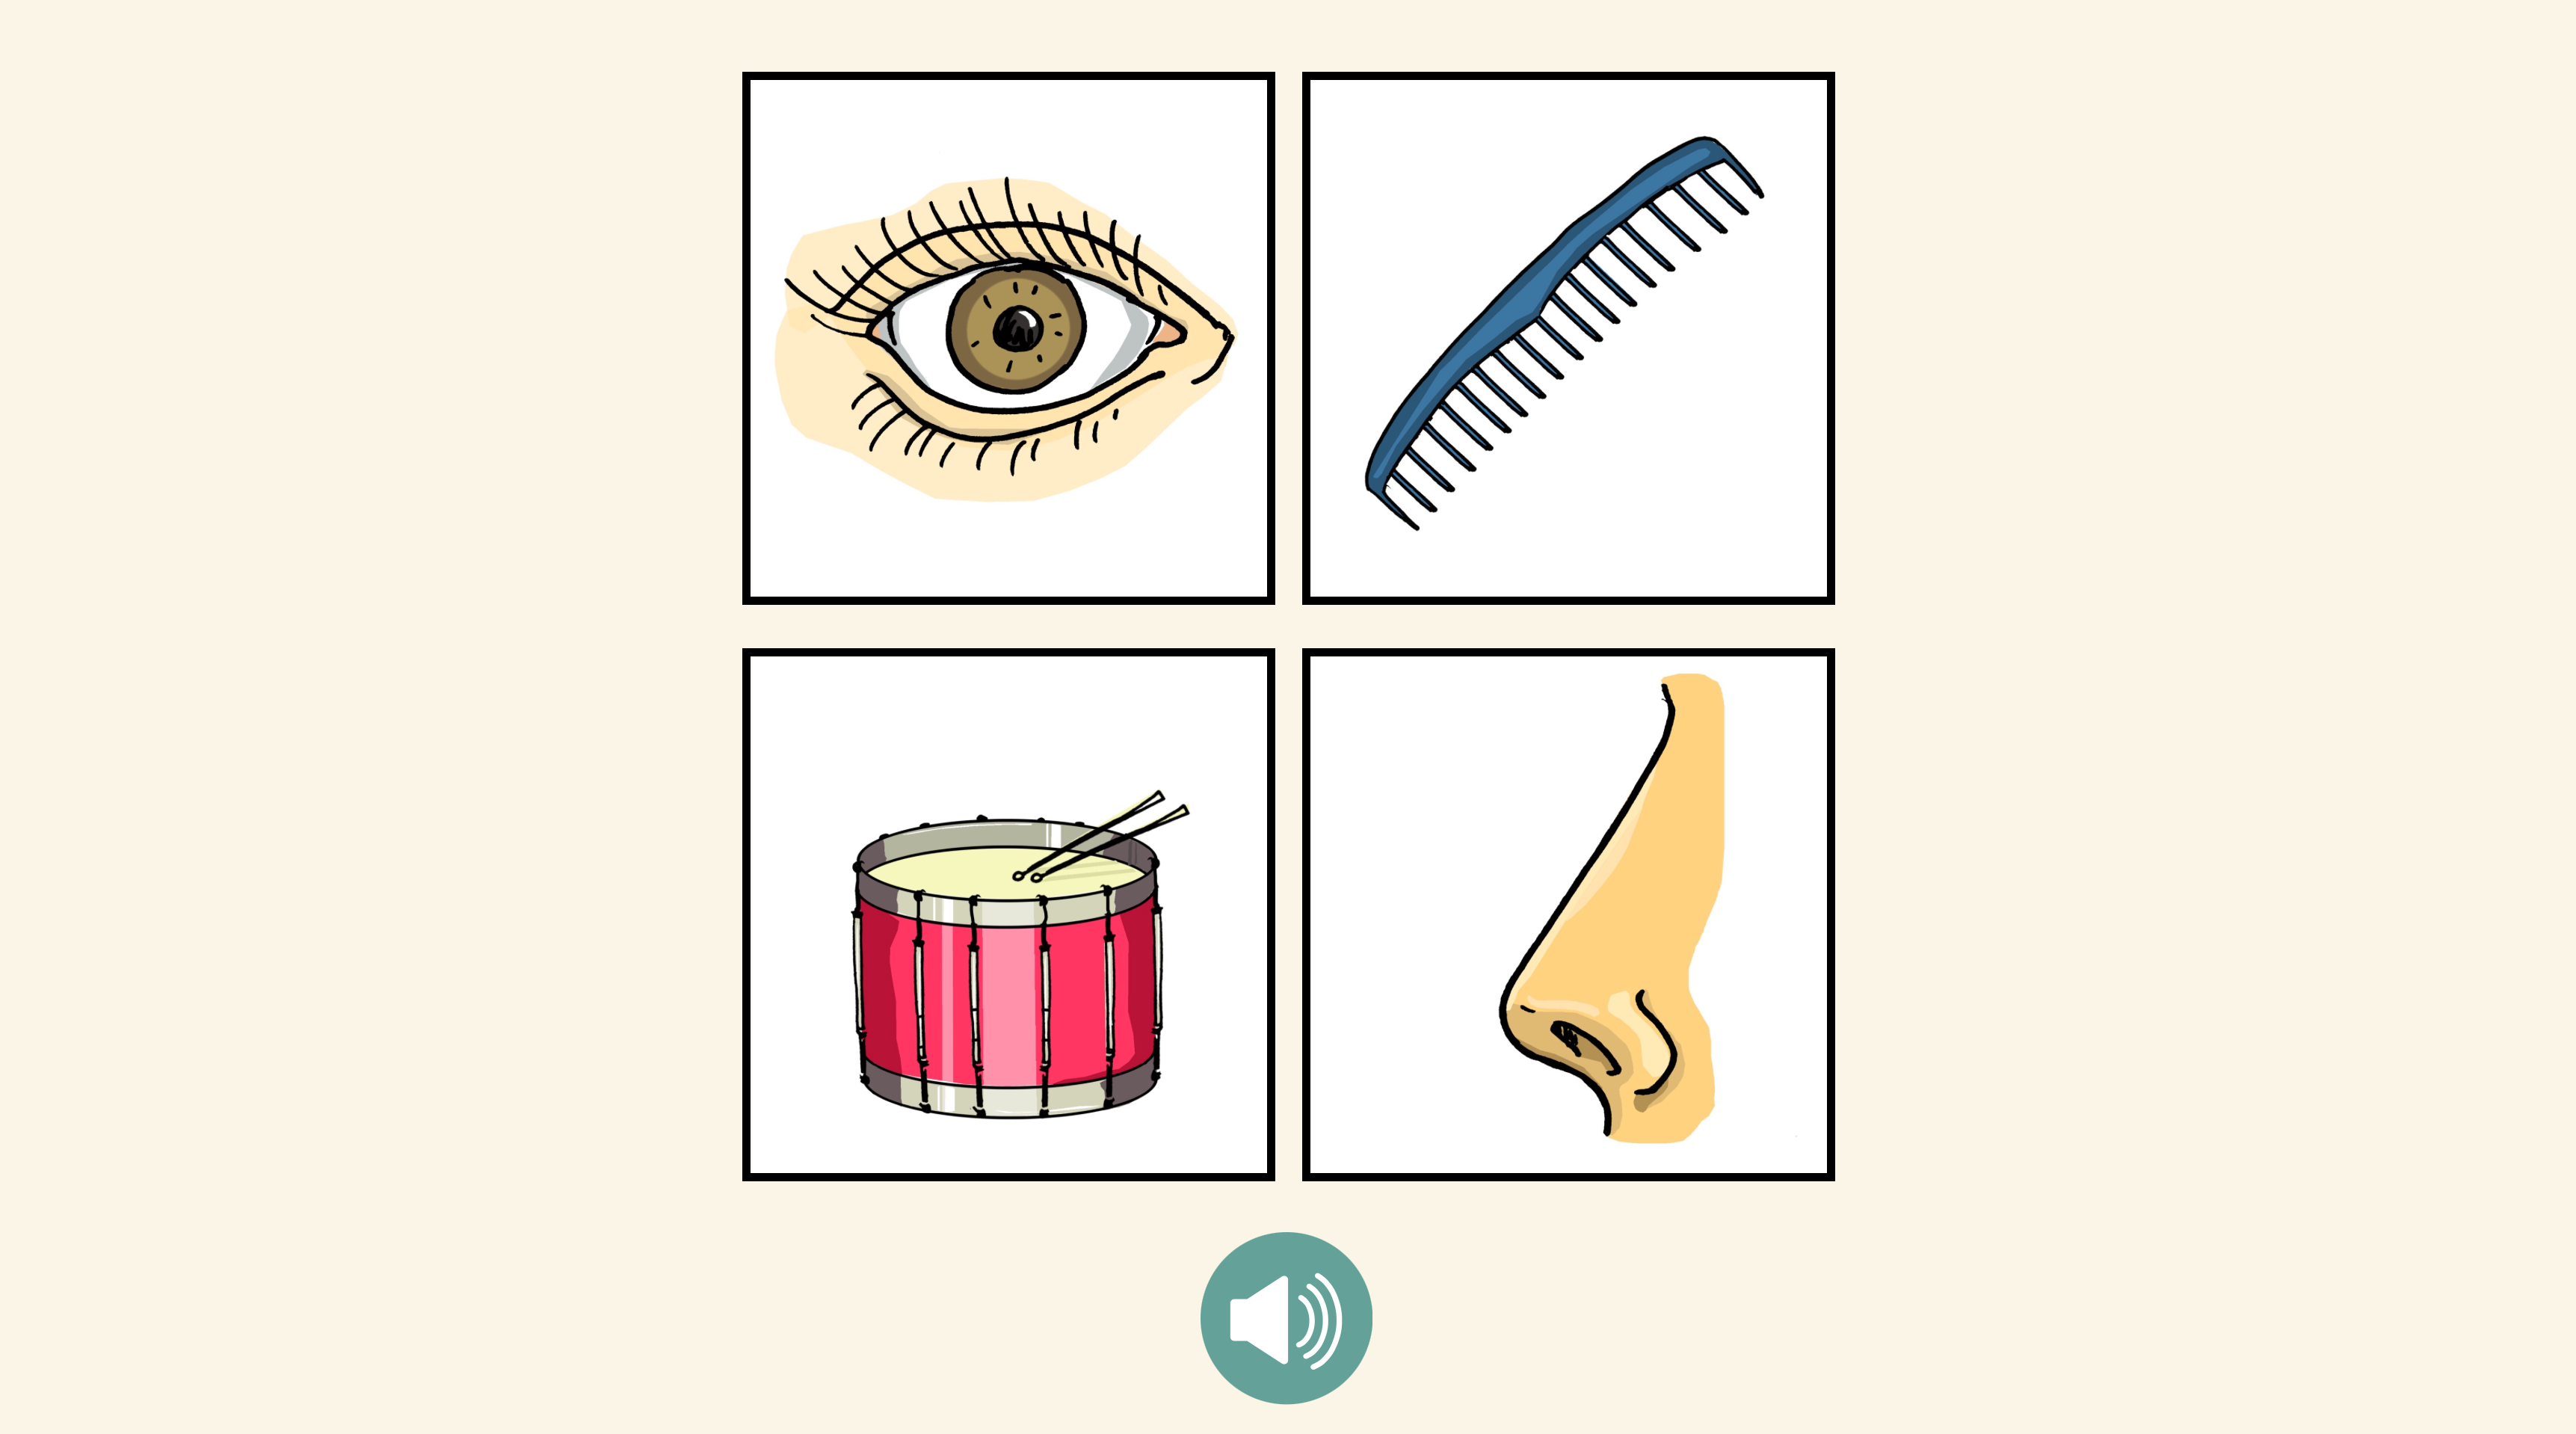
\includegraphics[width=1\linewidth]{../figures/orev} 

}

\caption{*OREV procedure**. Test for a figure caption.}\label{fig:fig1}
\end{figure}

Lorem ipsum dolor sit amet, consectetur adipiscing elit, sed do eiusmod tempor incididunt ut labore et dolore magna aliqua. Luctus venenatis lectus magna fringilla urna. Laoreet non curabitur gravida arcu ac tortor. Faucibus vitae aliquet nec ullamcorper sit amet risus nullam eget. Cras semper auctor neque vitae tempus quam pellentesque. Imperdiet massa tincidunt nunc pulvinar sapien et ligula ullamcorper. Et tortor at risus viverra adipiscing at. Congue nisi vitae suscipit tellus mauris. Habitant morbi tristique senectus et netus et malesuada fames ac. Eget mauris pharetra et ultrices neque. Aenean et tortor at risus viverra. Tempor orci dapibus ultrices in iaculis nunc sed augue. Euismod lacinia at quis risus sed vulputate odio ut enim. Id eu nisl nunc mi ipsum faucibus. Est lorem ipsum dolor sit amet. Eget velit aliquet sagittis id consectetur purus. Faucibus ornare suspendisse sed nisi. Pellentesque diam volutpat commodo sed egestas egestas fringilla.

Facilisi morbi tempus iaculis urna id volutpat. Faucibus in ornare quam viverra orci sagittis eu volutpat odio. Commodo elit at imperdiet dui. Condimentum mattis pellentesque id nibh tortor id aliquet lectus. Quis vel eros donec ac odio. Condimentum id venenatis a condimentum vitae sapien pellentesque habitant. Laoreet sit amet cursus sit amet dictum sit. Purus faucibus ornare suspendisse sed. Ornare arcu dui vivamus arcu. Scelerisque fermentum dui faucibus in. Nulla aliquet porttitor lacus luctus accumsan tortor posuere. Donec adipiscing tristique risus nec feugiat. Vitae turpis massa sed elementum tempus. Quis vel eros donec ac odio tempor. Iaculis eu non diam phasellus vestibulum lorem. Id porta nibh venenatis cras sed felis. Facilisi cras fermentum odio eu feugiat.

Lobortis feugiat vivamus at augue. Dignissim enim sit amet venenatis urna. Elementum sagittis vitae et leo duis ut diam quam. At lectus urna duis convallis convallis. Nisl condimentum id venenatis a condimentum vitae sapien pellentesque habitant. Mauris pellentesque pulvinar pellentesque habitant morbi tristique. Elit at imperdiet dui accumsan sit amet nulla facilisi morbi. Leo integer malesuada nunc vel risus commodo. Risus nec feugiat in fermentum posuere urna nec tincidunt. Quam id leo in vitae turpis massa. Duis ut diam quam nulla porttitor massa. Sem viverra aliquet eget sit amet tellus cras. Id nibh tortor id aliquet lectus proin nibh. Senectus et netus et malesuada fames ac. Leo urna molestie at elementum eu facilisis sed. Bibendum enim facilisis gravida neque convallis. Aenean vel elit scelerisque mauris pellentesque. Vitae purus faucibus ornare suspendisse.

Mauris nunc congue nisi vitae suscipit. Aenean euismod elementum nisi quis eleifend quam. Sed tempus urna et pharetra pharetra massa massa ultricies mi. Urna porttitor rhoncus dolor purus non. Rutrum tellus pellentesque eu tincidunt tortor. Fringilla urna porttitor rhoncus dolor purus non enim praesent. Tellus in hac habitasse platea dictumst vestibulum rhoncus est. Consectetur adipiscing elit pellentesque habitant. Et ligula ullamcorper malesuada proin libero. Viverra ipsum nunc aliquet bibendum enim.

In aliquam sem fringilla ut morbi tincidunt augue interdum. Rutrum quisque non tellus orci ac auctor augue mauris augue. Amet tellus cras adipiscing enim eu turpis egestas pretium. Nisl tincidunt eget nullam non nisi est sit amet facilisis. Diam quis enim lobortis scelerisque fermentum dui faucibus. Magna ac placerat vestibulum lectus mauris ultrices eros. Ac turpis egestas maecenas pharetra convallis posuere morbi leo. Velit aliquet sagittis id consectetur purus. Semper quis lectus nulla at volutpat diam. Orci nulla pellentesque dignissim enim sit amet venenatis urna. Lorem dolor sed viverra ipsum nunc. Risus nullam eget felis eget. Maecenas accumsan lacus vel facilisis. Sem integer vitae justo eget magna. Ac ut consequat semper viverra nam libero. Faucibus interdum posuere lorem ipsum dolor sit amet. Faucibus scelerisque eleifend donec pretium vulputate sapien nec. Leo vel fringilla est ullamcorper eget.

Euismod in pellentesque massa placerat. Volutpat diam ut venenatis tellus in metus vulputate eu scelerisque. Commodo quis imperdiet massa tincidunt nunc pulvinar sapien et. Vulputate dignissim suspendisse in est ante in nibh mauris. Proin fermentum leo vel orci porta non. Quis lectus nulla at volutpat diam ut venenatis tellus in. Leo vel orci porta non. Venenatis a condimentum vitae sapien pellentesque habitant morbi tristique. Quisque egestas diam in arcu. Vitae justo eget magna fermentum iaculis eu. Consequat ac felis donec et odio pellentesque diam. Nibh sed pulvinar proin gravida. Interdum consectetur libero id faucibus nisl tincidunt. Risus ultricies tristique nulla aliquet enim. Enim praesent elementum facilisis leo vel fringilla. Viverra nibh cras pulvinar mattis nunc. Lorem dolor sed viverra ipsum nunc aliquet bibendum enim. Interdum consectetur libero id faucibus nisl tincidunt eget. Faucibus purus in massa tempor nec feugiat nisl pretium. Ac auctor augue mauris augue neque gravida in fermentum et.

In ante metus dictum at tempor commodo ullamcorper a lacus. Arcu vitae elementum curabitur vitae nunc sed. Eu scelerisque felis imperdiet proin fermentum leo. Orci ac auctor augue mauris augue neque gravida. Ac tortor dignissim convallis aenean et tortor at. Non arcu risus quis varius quam quisque. Ultricies integer quis auctor elit sed. Sit amet risus nullam eget felis eget nunc. Urna condimentum mattis pellentesque id nibh tortor id. Aliquam vestibulum morbi blandit cursus. Viverra tellus in hac habitasse platea dictumst vestibulum rhoncus est. Quis lectus nulla at volutpat diam. Lacus luctus accumsan tortor posuere. Non sodales neque sodales ut etiam sit amet nisl purus.

Cras semper auctor neque vitae tempus. Libero nunc consequat interdum varius. Orci ac auctor augue mauris augue neque gravida in. Ut placerat orci nulla pellentesque dignissim enim sit amet venenatis. Nunc mi ipsum faucibus vitae aliquet nec ullamcorper sit amet. Tortor dignissim convallis aenean et tortor at. Facilisi nullam vehicula ipsum a arcu cursus vitae. Felis imperdiet proin fermentum leo vel. Blandit volutpat maecenas volutpat blandit. Tortor id aliquet lectus proin. Enim eu turpis egestas pretium. Nunc faucibus a pellentesque sit amet porttitor. Fermentum iaculis eu non diam phasellus vestibulum. Porta lorem mollis aliquam ut porttitor. Amet nisl suscipit adipiscing bibendum. Malesuada fames ac turpis egestas integer eget aliquet nibh praesent. Libero volutpat sed cras ornare arcu. Arcu cursus euismod quis viverra nibh cras pulvinar mattis nunc. Lacinia quis vel eros donec ac odio tempor orci. Lacinia quis vel eros donec ac.

Varius duis at consectetur lorem donec massa sapien faucibus. Ac auctor augue mauris augue neque gravida in fermentum. Pellentesque habitant morbi tristique senectus et. Turpis egestas sed tempus urna et pharetra. Vitae auctor eu augue ut lectus. Est lorem ipsum dolor sit. Eget nunc lobortis mattis aliquam faucibus purus in massa. Donec ultrices tincidunt arcu non sodales neque. Sollicitudin nibh sit amet commodo nulla. Magna ac placerat vestibulum lectus mauris ultrices eros in. Sem viverra aliquet eget sit. Pellentesque massa placerat duis ultricies lacus sed turpis. Facilisi morbi tempus iaculis urna id volutpat lacus laoreet non. Massa massa ultricies mi quis. Aenean euismod elementum nisi quis eleifend quam adipiscing vitae. Ultrices eros in cursus turpis massa tincidunt dui. Augue lacus viverra vitae congue eu consequat. Eros in cursus turpis massa tincidunt dui. Facilisi morbi tempus iaculis urna id. Feugiat nibh sed pulvinar proin gravida hendrerit lectus a.

Mattis pellentesque id nibh tortor id aliquet lectus proin nibh. A cras semper auctor neque vitae tempus. Est pellentesque elit ullamcorper dignissim. Nulla facilisi etiam dignissim diam quis enim lobortis scelerisque fermentum. Laoreet sit amet cursus sit. Etiam tempor orci eu lobortis elementum nibh tellus molestie nunc. Nunc vel risus commodo viverra maecenas. Duis ut diam quam nulla porttitor. Ornare arcu odio ut sem nulla. Magna etiam tempor orci eu lobortis. Porttitor lacus luctus accumsan tortor posuere. Natoque penatibus et magnis dis parturient. Velit ut tortor pretium viverra suspendisse potenti nullam ac. Morbi leo urna molestie at. Nascetur ridiculus mus mauris vitae ultricies leo integer malesuada nunc. Sed viverra ipsum nunc aliquet bibendum enim facilisis gravida.

Risus ultricies tristique nulla aliquet enim tortor at auctor urna. Nisl rhoncus mattis rhoncus urna neque viverra justo nec ultrices. Id nibh tortor id aliquet lectus proin nibh nisl. Interdum varius sit amet mattis vulputate enim nulla aliquet porttitor. Ullamcorper eget nulla facilisi etiam. Scelerisque eleifend donec pretium vulputate sapien nec sagittis aliquam malesuada. Dui ut ornare lectus sit amet est placerat in egestas. Ultrices dui sapien eget mi proin. Sit amet nisl purus in mollis nunc. Senectus et netus et malesuada fames ac turpis. Nisi vitae suscipit tellus mauris a diam maecenas. Semper eget duis at tellus at urna condimentum.

Nibh nisl condimentum id venenatis. Ornare suspendisse sed nisi lacus sed viverra tellus in hac. Sed arcu non odio euismod lacinia. Sed libero enim sed faucibus turpis in eu mi. Dolor morbi non arcu risus quis varius quam quisque id. Etiam erat velit scelerisque in dictum non consectetur. Risus sed vulputate odio ut enim blandit volutpat maecenas volutpat. Libero volutpat sed cras ornare. Tellus cras adipiscing enim eu turpis egestas pretium aenean. Neque sodales ut etiam sit amet nisl.

A pellentesque sit amet porttitor eget dolor morbi. Libero volutpat sed cras ornare arcu dui vivamus arcu felis. Ultricies tristique nulla aliquet enim tortor at auctor. Tortor aliquam nulla facilisi cras fermentum odio eu feugiat. Natoque penatibus et magnis dis parturient montes nascetur. Ullamcorper eget nulla facilisi etiam dignissim diam quis enim. Sed elementum tempus egestas sed. Elementum eu facilisis sed odio morbi quis commodo. Proin fermentum leo vel orci. Id porta nibh venenatis cras sed felis eget velit. Vitae semper quis lectus nulla at volutpat.

Dictum fusce ut placerat orci nulla pellentesque dignissim enim. Turpis egestas sed tempus urna et pharetra pharetra massa. Pellentesque elit eget gravida cum sociis. Pellentesque id nibh tortor id aliquet lectus proin. Consectetur lorem donec massa sapien faucibus et molestie. Ut tellus elementum sagittis vitae et leo. Nisl condimentum id venenatis a condimentum vitae sapien pellentesque. A pellentesque sit amet porttitor eget dolor. In egestas erat imperdiet sed. Nec dui nunc mattis enim ut tellus elementum. Ut pharetra sit amet aliquam id diam maecenas ultricies mi. Massa enim nec dui nunc mattis enim. Nisl condimentum id venenatis a condimentum vitae sapien.

Habitasse platea dictumst vestibulum rhoncus est pellentesque. Tincidunt augue interdum velit euismod in pellentesque. Feugiat in fermentum posuere urna nec tincidunt. Tortor at auctor urna nunc id cursus metus aliquam. Pulvinar etiam non quam lacus. Imperdiet sed euismod nisi porta. Rhoncus urna neque viverra justo nec ultrices dui sapien eget. Ligula ullamcorper malesuada proin libero nunc consequat interdum varius sit. Mi ipsum faucibus vitae aliquet nec ullamcorper sit amet risus. Eu lobortis elementum nibh tellus molestie nunc. In est ante in nibh mauris cursus mattis molestie a. Sagittis id consectetur purus ut faucibus pulvinar elementum. Et netus et malesuada fames ac turpis egestas sed. Bibendum at varius vel pharetra vel turpis nunc eget lorem. Sem et tortor consequat id porta nibh venenatis cras sed. At urna condimentum mattis pellentesque.

\section{Social Cognition}\label{social-cognition}

\section{Gaze Following}\label{gaze-following}

\section{Methodological Considerations}\label{methodological-considerations}

\chapter{This Dissertation}\label{aims}

\section{Research Focus}\label{research-focus}

\section{Study Populations}\label{study-populations}

\section{Aims and Approaches}\label{aims-and-approaches}

\section{Ethics Statement}\label{ethics-statement}

\chapter{Results}\label{results}

\chapter{General Discussion}\label{discussion}

\backmatter

\chapter{References}\label{references}

\phantomsection\label{refs}
\begin{CSLReferences}{1}{0}
\bibitem[\citeproctext]{ref-prein2023tango}
Prein, J. C., Kalinke, S., Haun, D. B. M., \& Bohn, M. (2023). {TANGO}: {A} reliable, open-source, browser-based task to assess individual differences in gaze understanding in 3 to 5-year-old children and adults. \emph{Behavior Research Methods}, \emph{56}(3), 2469--2485. \url{https://doi.org/10.3758/s13428-023-02159-5}

\end{CSLReferences}

\chapter{Appendix A --- Main Publications}\label{appendixA}

This dissertation includes four main publications that were either published (\hyperref[studyI]{Study I}) or under review (\hyperref[studyII]{Study II}, \hyperref[studyIII]{Study III}, \hyperref[studyIV]{Study IV}) at the time of the dissertation submission. The full texts of these publications are provided below. For the accepted manuscript, the published version is provided. For manuscripts under review, the submitted versions are provided which are published online as pre-prints.

~

\textbf{\hyperref[studyI]{Study I}:} Prein, J. C., Kalinke, S., Haun, D. B. M.*, \& Bohn, M.* (2023). TANGO: A reliable, open-source, browser-based task to assess individual differences in gaze understanding in 3 to 5-year-old children and adults. \emph{Behavior Research Methods, 56}(3), 2469--2485. \url{https://doi.org/10.3758/s13428-023-02159-5}

\textbf{\hyperref[studyII]{Study II}:} Prein, J. C., Maurits, L., Werwach, A., Haun, D. B. M.,* \& Bohn, M.* (2024). \emph{Variation in gaze understanding across the life span: A process-level perspective.} PsyArXiv. \url{https://doi.org/10.31234/osf.io/dy73a}

\textbf{\hyperref[studyIII]{Study III}:} Bohn, M.*, Prein, J. C.*, Ayikoru, A., Bednarski, F. M., Dzabatou, A., Frank, M. C., Henderson, A. M. E., Isabella, J., Kalbitz, J., Kanngiesser, P., Keşşafoğlu, D., Koymen, B., Manrique-Hernandez, M., Magazi, S., Mújica-Manrique, L., Ohlendorf, J., Olaoba, D., Pieters, W., Pope-Caldwell, S., \ldots{} Haun, D. (2024). \emph{A universal of human social cognition: Children from 17 communities process gaze in similar ways.} PsyArXiv. \url{https://doi.org/10.31234/osf.io/z3ahv}

\textbf{\hyperref[studyIV]{Study IV}:} Prein, J. C., Maurits, L., Werwach, A., Haun, D. B. M., \& Bohn, M. (2024). \emph{Variation in gaze following across the life span: A process-level perspective.} PsyArXiv. \url{https://doi.org/10.31234/osf.io/dy73a}

\newpage

\section{Study I}\label{studyI}

\begin{minipage}{\textwidth}
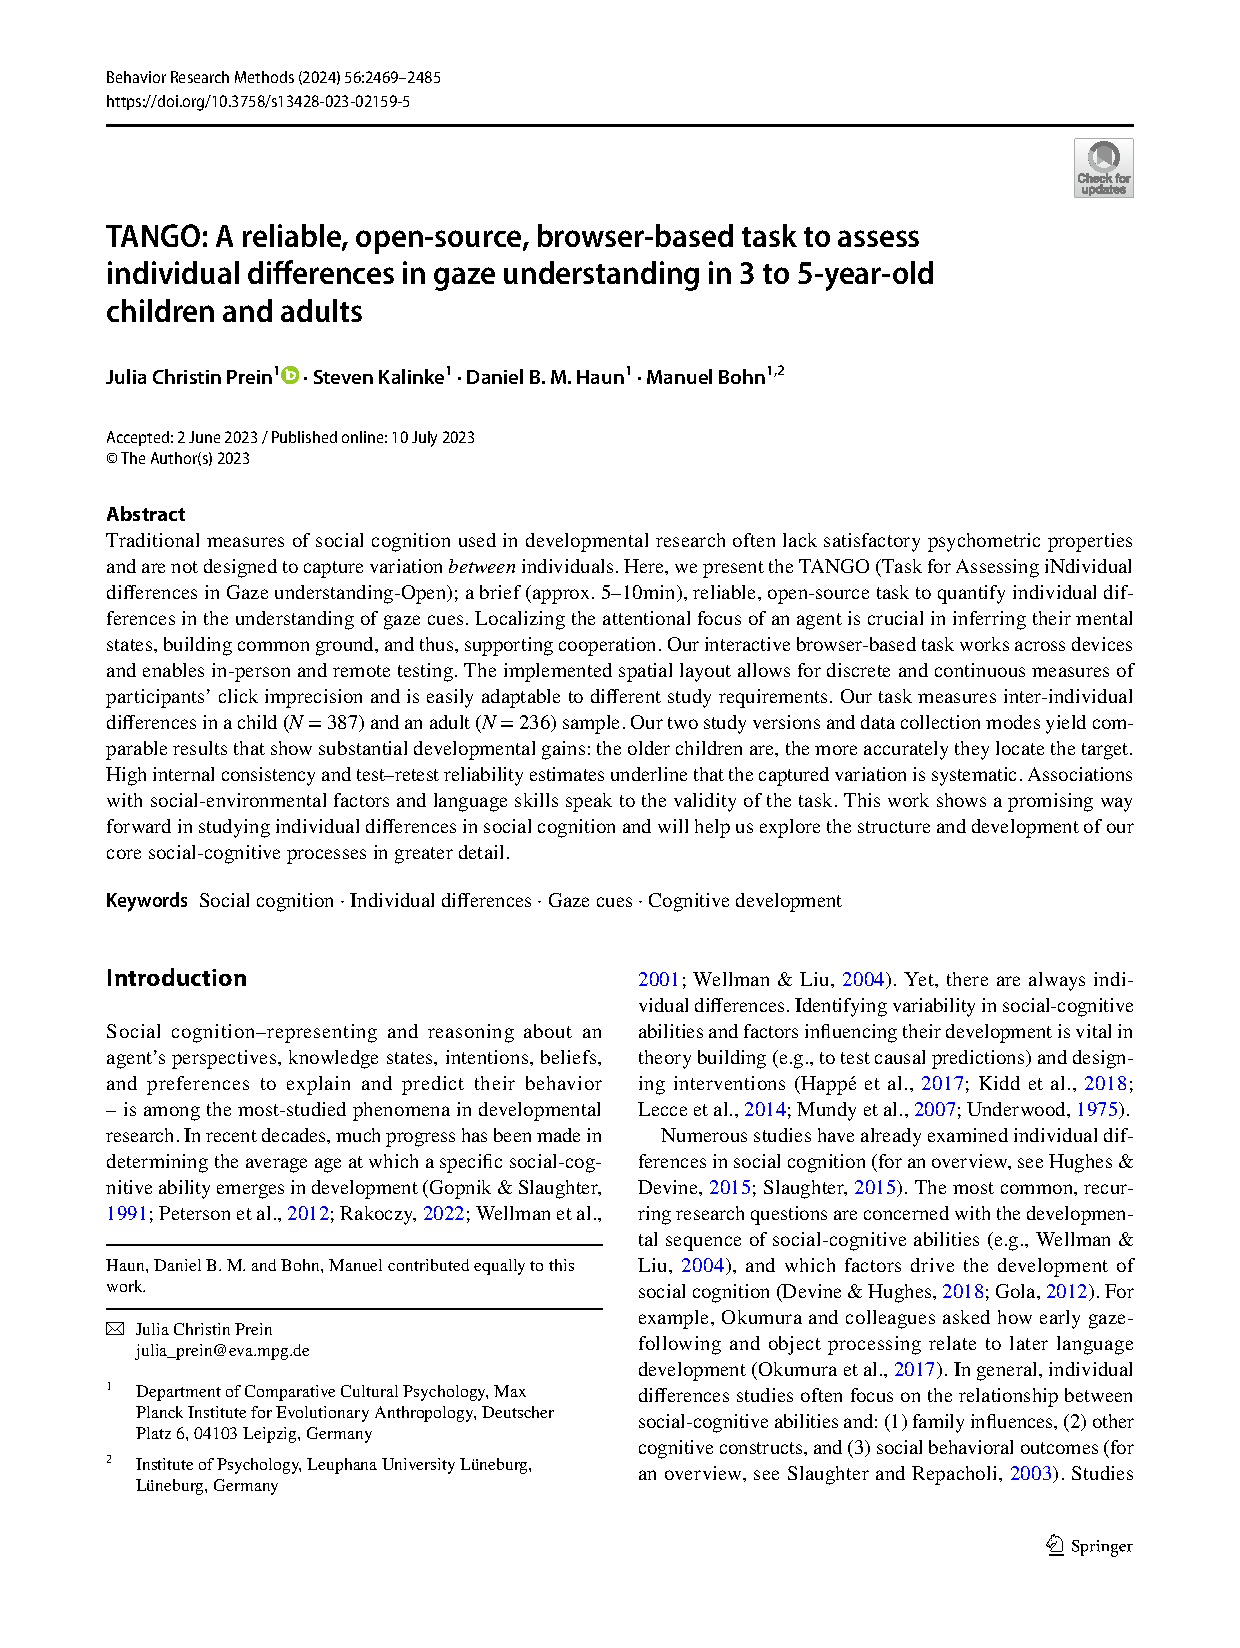
\includepdf[pages={1}, scale=0.85, offset=0 -1cm, pagecommand={}]{../papers/studyI.pdf}
\end{minipage}

\includepdf[pages={2-}, scale=0.85, pagecommand={}]{../papers/studyI.pdf}

\newpage

\section{Study II}\label{studyII}

\begin{minipage}{\textwidth}
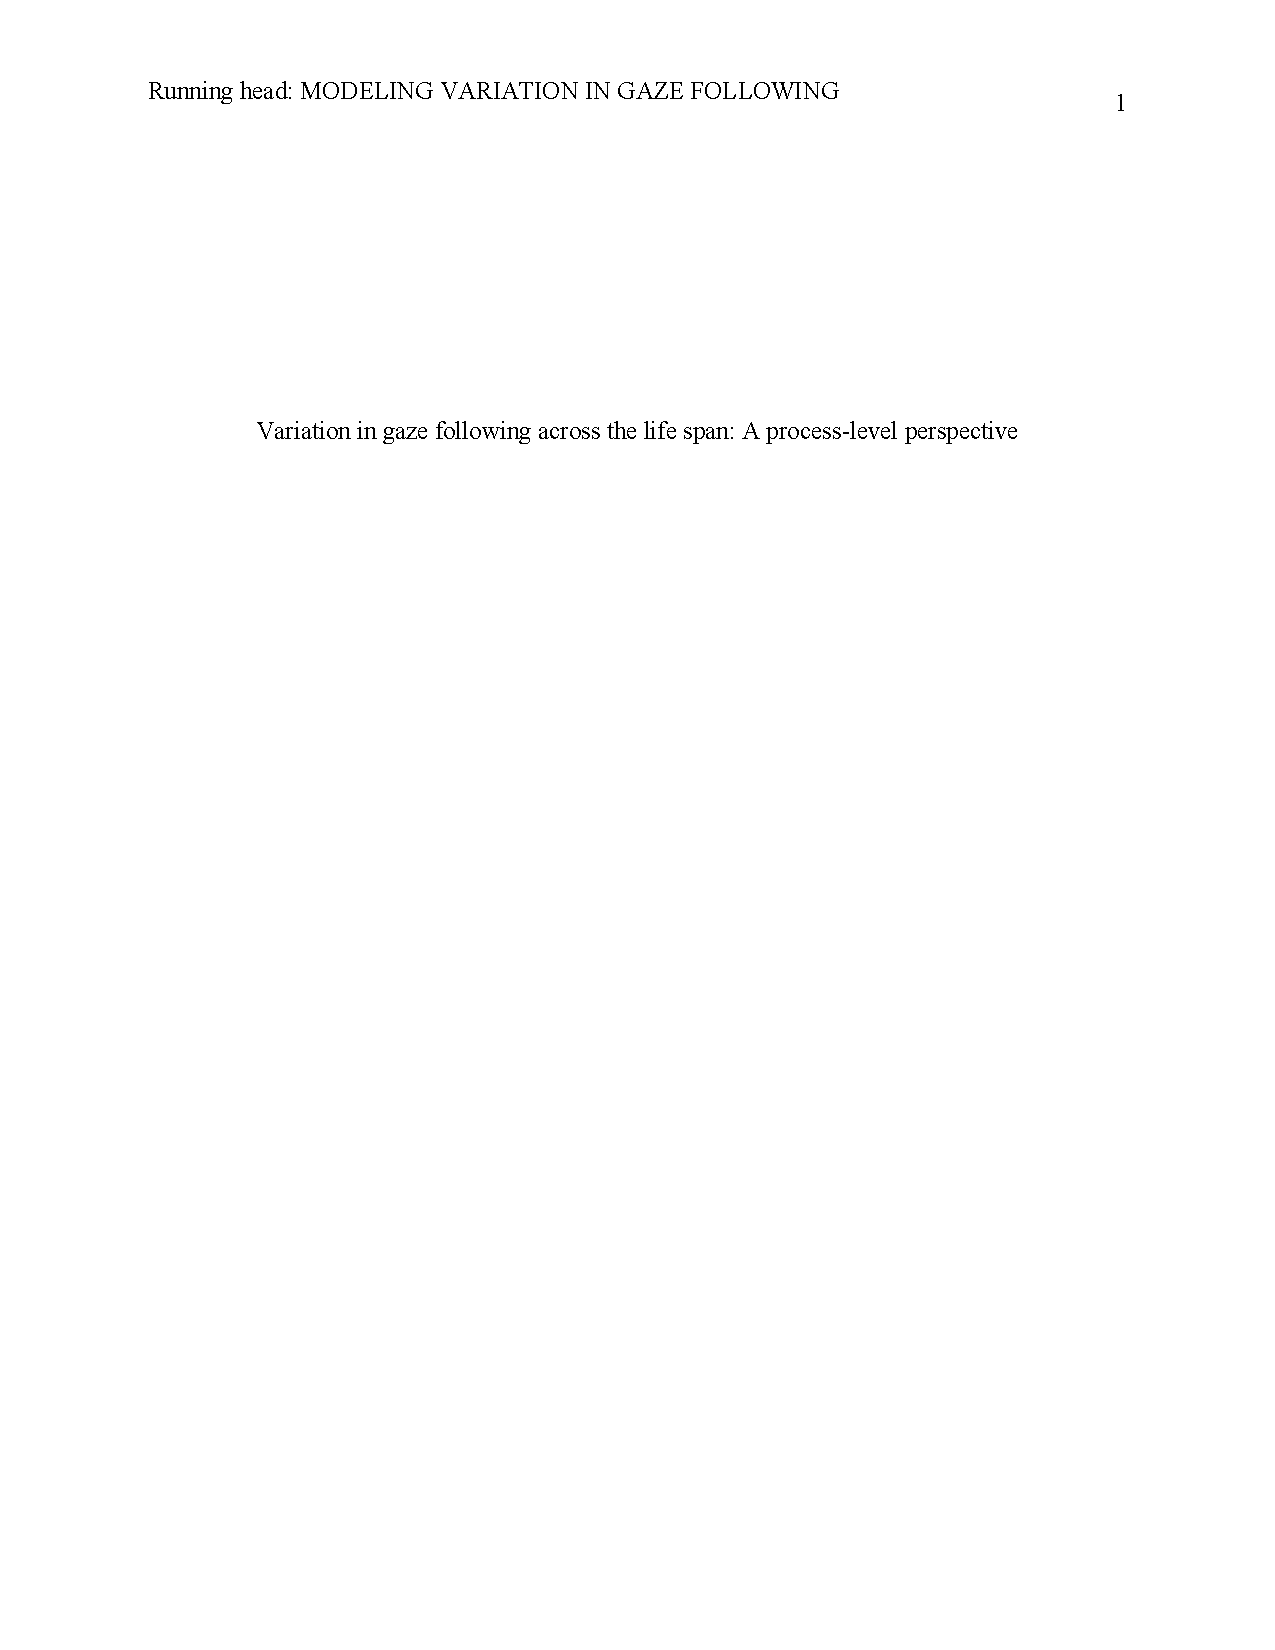
\includepdf[pages={1}, scale=0.85, offset=0 -1cm, pagecommand={}]{../papers/studyII.pdf}
\end{minipage}

\includepdf[pages={2-}, scale=0.85, pagecommand={}]{../papers/studyII.pdf}

\newpage

\section{Study III}\label{studyIII}

\begin{minipage}{\textwidth}
\includepdf[pages={1}, scale=0.85, offset=0 -1cm, pagecommand={}]{../papers/studyIII.pdf}
\end{minipage}

\includepdf[pages={2-}, scale=0.85, pagecommand={}]{../papers/studyIII.pdf}

\newpage

\section{Study IV}\label{studyIV}

\begin{minipage}{\textwidth}
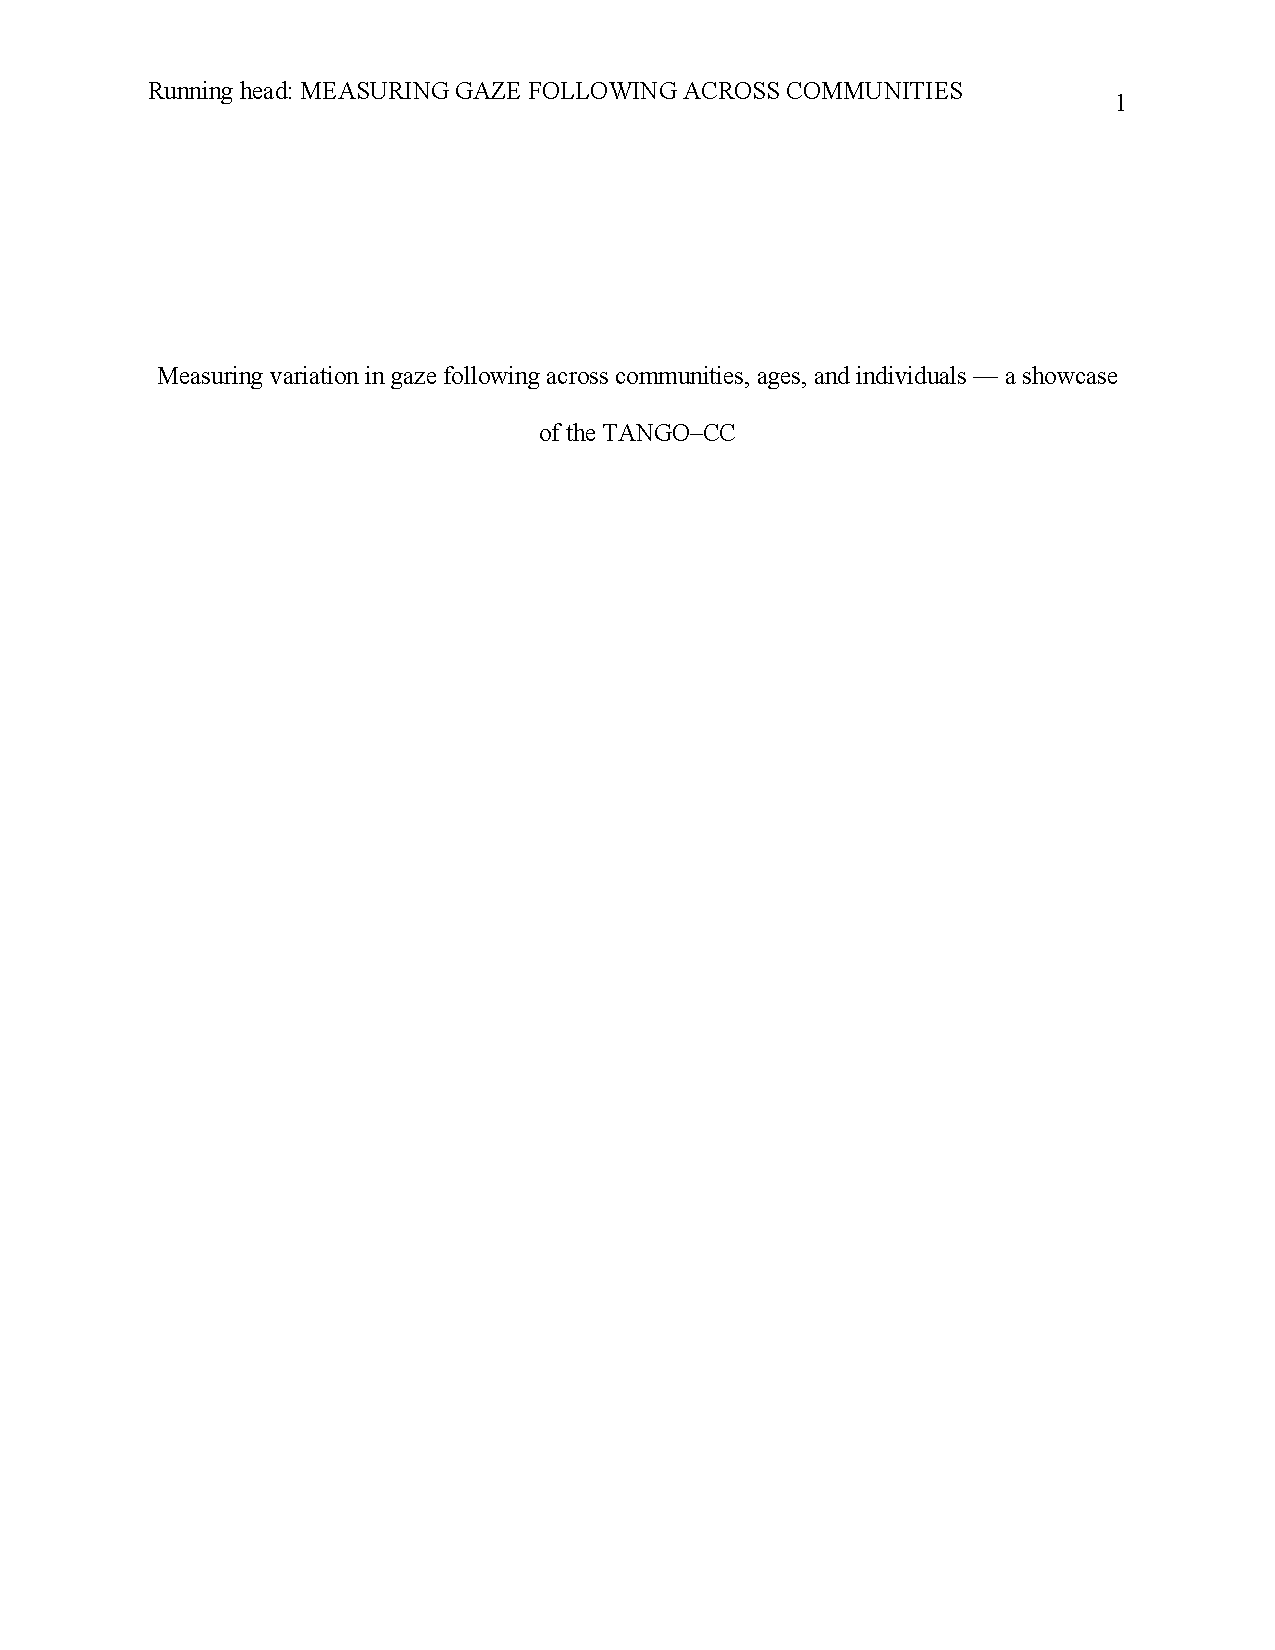
\includepdf[pages={1}, scale=0.85, offset=0 -1cm, pagecommand={}]{../papers/studyIV.pdf}
\end{minipage}

\includepdf[pages={2-}, scale=0.85, pagecommand={}]{../papers/studyIV.pdf}

\chapter{Appendix B --- Further Publications}\label{appendixB}

The following Appendix B contains other publications that were written in the context of the dissertation but not included in the main text, with their respective abstracts.

\section{Action anticipation based on an agent's epistemic state in toddlers and adults}\label{action-anticipation-based-on-an-agents-epistemic-state-in-toddlers-and-adults}

\textbf{Citation:} Schuwerk, T., Kampis, D., Baillargeon, R., Biro, S., Bohn, M., Byers-Heinlein, K., Dörrenberg, S., Fisher, C., Franchin, L., Fulcher, T., Garbisch, I., Geraci, A., Grosse Wiesmann, C., Hamlin, K., Haun, D. B. M., Hepach, R., Hunnius, S., Hyde, D. C., Karman, P., \ldots, Prein, J., \ldots{} Rakoczy, H. (2021). \emph{Action anticipation based on an agent's epistemic state in toddlers and adults. Child Development} (In-Principle Acceptance of Registered Report Stage 1: Study Design). PsyArXiv. \url{https://doi.org/10.31234/osf.io/x4jbm}

\textbf{Abstract:} Do toddlers and adults engage in spontaneous Theory of Mind (ToM)? Evidence from anticipatory looking (AL) studies suggests that they do. But a growing body of failed replication studies raised questions about the paradigm's suitability. In this multi-lab collaboration, we test the robustness of spontaneous ToM measures. We examine whether 18- to 27-month-olds' and adults' anticipatory looks distinguish between two basic forms of an agent's epistemic states: knowledge and ignorance. In toddlers {[}ANTICIPATED n = 520 50\% FEMALE{]} and adults {[}ANTICIPATED n = 408, 50\% FEMALE{]} from diverse ethnic backgrounds, we found {[}SUPPORT/NO SUPPORT{]} for epistemic state-based action anticipation. Future research can probe whether this conclusion extends to more complex kinds of epistemic states, such as true and false beliefs.

\emph{Please note that this abstract was written for the Registered Report and does not entail results yet. Text in square brackets indicates placeholder text to be filled in after data collection.}

\newpage

\section{PREVIC: An adaptive parent report measure of expressive vocabulary in children between 3 and 8 years of age}\label{previc-an-adaptive-parent-report-measure-of-expressive-vocabulary-in-children-between-3-and-8-years-of-age}

\textbf{Citation:} Bohn, M., Prein, J. C., Engicht, J., Haun, D., Gagarina, N., \& Koch, T. (2023). \emph{PREVIC: An adaptive parent report measure of expressive vocabulary in children between 3 and 8 years of age.} PsyArXiv. \url{https://doi.org/10.31234/osf.io/hvncp}

\textbf{Abstract:} Parent report measures have proven to be a valuable research tool to study early language development. Caregivers are given a list of words and are asked which of them their child has already used. However, most available measures are not suited for children beyond infancy, come with substantial licensing costs or lack a clear psychometric foundation. Here we present the PREVIC (Parent Report of Expressive Vocabulary in Children), an open access, high quality vocabulary checklist for German-speaking children between three and eight years of age. The PREVIC was constructed leveraging the advantages of Item Response Theory: we designed a large initial item pool of 379 words and collected data from N = 1190 caregivers of children between three and eight years of age. Based on this data, we computed a range of fit indices for each item (word) and used an automated item selection algorithm to compile a final pool that contains items that a) vary in difficulty and b) fit the Rasch (one-parameter logistic) model. The resulting task is highly reliable and shows convergent validity. The IRT-based construction allowed us to design an adaptive version of the task, which substantially reduces the duration of the task while retaining measurement precision. The task -- including the adaptive version -- was implemented as a website and is freely accessible online (\url{https://ccp-odc.eva.mpg.de/previc-demo/}). The PREVIC fills an important gap in the toolkit of researchers interested in language development and provides an ideal starting point for the development of converging measures in other languages.

\newpage

\section{oREV: An item response theory-based open receptive vocabulary task for 3- to 8-year-old children}\label{orev-an-item-response-theory-based-open-receptive-vocabulary-task-for-3--to-8-year-old-children}

\textbf{Citation:} Bohn, M.*, Prein, J.*, Koch, T., Bee, R. M., Delikaya, B., Haun, D., \& Gagarina, N. (2024). oREV: An item response theory-based open receptive vocabulary task for 3- to 8-year-old children. \emph{Behavior Research Methods, 56}(3), 2595--2605. \url{https://doi.org/10.3758/s13428-023-02169-3}

\textbf{Abstract:} Individual differences in early language abilities are an important predictor of later life outcomes. High-quality, easy-access measures of language abilities are rare, especially in the preschool and primary school years. The present study describes the construction of a new receptive vocabulary task for children between 3 and 8 years of age. The task was implemented as a browser-based web application, allowing for both in-person and remote data collection via the internet. Based on data from N = 581 German-speaking children, we estimated the psychometric properties of each item in a larger initial item pool via item response modeling. We then applied an automated item selection procedure to select an optimal subset of items based on item difficulty and discrimination. The so-constructed task has 22 items and shows excellent psychometric properties with respect to reliability, stability, and convergent and discriminant validity. The construction, implementation, and item selection process described here makes it easy to extend the task or adapt it to different languages. All materials and code are freely accessible to interested researchers. The task can be used via the following website: \url{https://ccp-odc.eva.mpg.de/orev-demo}.

\newpage

\section{Validation of an open source, remote web-based eye-tracking method (WebGazer) for research in early childhood}\label{validation-of-an-open-source-remote-web-based-eye-tracking-method-webgazer-for-research-in-early-childhood}

\textbf{Citation:} Steffan, A., Zimmer, L., Arias-Trejo, N., Bohn, M., Dal Ben, R., Flores-Coronado, M. A., Franchin, L., Garbisch, I., Grosse Wiesmann, C., Hamlin, J. K., Havron, N., Hay, J. F., Hermansen, T. K., Jakobsen, K. V., Kalinke, S., Ko, E.-S., Kulke, L., Mayor, J., Meristo, M., \ldots, Prein, J., \ldots, Schuwerk, T. (2024). Validation of an open source, remote web-based eye-tracking method (WebGazer) for research in early childhood. \emph{Infancy, 29}(1), 31--55. \url{https://doi.org/10.1111/infa.12564}

\textbf{Abstract:} Measuring eye movements remotely via the participant's webcam promises to be an attractive methodological addition to in-person eye-tracking in the lab. However, there is a lack of systematic research comparing remote web-based eye-tracking with in-lab eye-tracking in young children. We report a multi-lab study that compared these two measures in an anticipatory looking task with toddlers using WebGazer.js and jsPsych. Results of our remotely tested sample of 18-27-month-old toddlers (N = 125) revealed that web-based eye-tracking successfully captured goal-based action predictions, although the proportion of the goal-directed anticipatory looking was lower compared to the in-lab sample (N = 70). As expected, attrition rate was substantially higher in the web-based (42\%) than the in-lab sample (10\%). Excluding trials based on visual inspection of the match of time-locked gaze coordinates and the participant's webcam video overlayed on the stimuli was an important preprocessing step to reduce noise in the data. We discuss the use of this remote web-based method in comparison with other current methodological innovations. Our study demonstrates that remote web-based eye-tracking can be a useful tool for testing toddlers, facilitating recruitment of larger and more diverse samples; a caveat to consider is the larger drop-out rate.

\chapter{Appendix C}\label{appendixC}

\chapter{Selbstständigkeitserklärung}\label{selbststaendigkeit}

Julia Christin Prein\\
{[}Straße Hausnummer{]}\\
{[}PLZ Ort{]}\\
{[}Telefon{]}\\
{[}Email{]}\\

Hiermit erkläre ich, dass ich mich noch keiner Doktorprüfung unterzogen oder mich um Zulassung zu einer solchen beworben habe.

Ich versichere, dass die Dissertation {[}TODO: Titel Dissertation{]} in der gegenwärtigen oder einer anderen Fassung noch keiner anderen Hochschule zur Begutachtung vorgelegen hat.

Ich versichere an Eides statt, dass ich die eingereichte Dissertation {[}TODO: Titel Dissertation{]} selbstständig und ohne zulässige fremde Hilfe verfasst habe. Anderer als der von mir angegebenen Hilfsmittel und Schriften habe ich mich nicht bedient. Alle wörtlich oder sinngemäß anderen Schriften entnommenen Stellen habe ich kenntlich gemacht. Über die strafrechtlichen Folgen gemäß § 156 Strafgesetzbuch wurde ich in Kenntnis gesetzt.

~

{[}Ort{]}, {[}Datum{]} ~ ~ {[}Unterschrift{]}

\end{document}
